\chapter{Grundlagen}
\label{cha:Grundlagen}

Zunächst werden in Abschnitt \ref{sec:Thermodynamik} die Thermodynamik und die Komponenten eines Kaltdampfprozesses vorgestellt. 


\section{Kaltdampf-Kälteprozesses}
\label{sec:Thermodynamik}

\subsection*{Thermodynamik}
Ein Verdampfer hat die Aufgabe, einer Umgebung Wärme zu entziehen. Hierfür wird in einem Wärmeübertrager flüssiges Kältemittel verdampft. Das verdampfende Kältemittel kühlt zunächst den Wärmeübertrager, danach wird über die Wärmeübertrager-Lamellen der vorbei strömende Luft Wärme entzogen.
Der Kaltdampf-Kälteprozess ist ein linksläufiger \textit{Clausius-Rankine-Kreisprozess}. Die Zustandspunkte des verwendeten Kältemittels im log p,h Diagramm sind in Abbildung \ref{fig:Komponenten} dargestellt. 

\begin{figure}[htb]
\centering		
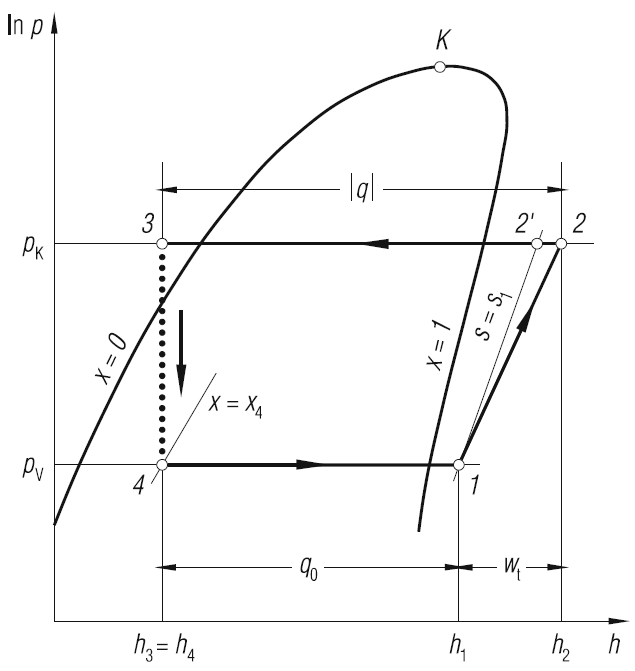
\includegraphics[width=0.6\textwidth]{Pictures/log_p_h_Beahr.png}
\caption{Kreisprozess im log p,h-Diagramm \citep{Baehr2013}}
\label{fig:Komponenten}
\end{figure}


Das halb-logarithmische Diagramm ist ein vielgebrauchtes und hilfreiches Mittel in der Kältetechnik. 
\footnote{Das Zustandsdiagramm wurde vom deutschen Ingenieur Richard Mollier (1863-1935) im Jahre 1924 erstmalig vorgestellt.} 
Der Druck ist logarithmisch auf der y-Achse und die spezifische Enthalpie $h$ auf der x-Achse eingetragen. Es gibt drei Gebiete im Diagramm: flüssiges Kältemittel, gasförmiges überhitztes Kältemittel und das Nassdampfgebiet. Im Nassdampfgebiet liegt ein Gemisch aus gasförmigen und flüssigem Kältemittel vor. Der Anteil des Gases im Nassdampfgebiet wird durch $x$ ausgedrückt; $1-x$ ist der Anteil der Flüssigkeit.


Im Diagramm \ref{fig:Komponenten} sind alle Zustandspunkte des Kältekreislaufes abgebildet. 
Innerhalb des Nassdampfgebietes führt Wärmezu- oder abfuhr  nicht zu einer Erhöhung der Temperatur, sondern zu einer Veränderung vom Gas- bzw. Flüssigkeitsanteil. Es wird von einer \textit{latenten}, also nicht fühlbaren,  Wärmeänderung gesprochen. 
%Um einen Tropfen flüssigen Wasser, dessen Zustand sich auf der Siedelinie befindet, in einen gasförmigen Zustand, sprich $x=1$ zu überführen, muss ihm die spezifische Verdampfungsenthalpie $\Delta h$ zugeführt werden. Verläuft die Zustandsänderung entgegengesetzt, kondensiert der Tropfen und gibt die Verdampfungsenthalpie $\Delta h$ an seine Umgebung ab. 
Außerhalb des Nassdampfgebietes führt eine Wärmezu- oder abfuhr zu einer Veränderung der Temperatur. Die Wärmeänderung ist \textit{sensibel}. 


Ein Kreisprozess kann in folgende vier Prozessschritte unterteilt werden:

\begin{tabular}{p{1.5cm}p{13cm}ll}
\hline
\textbf{1 $\longrightarrow$ 2} & Kompression des dampfförmigen Kältemittels durch mechanische Leistungszufuhr  \\ 
\hline
\textbf{2 $\longrightarrow$ 3} & Abkühlung, Kondensation und Unterkühlung des Kältemittels durch Abgabe vom Wärmestrom $\dot{Q}$ über den Verflüssiger an die Umgebung \\ 
\hline
\textbf{3 $\longrightarrow$ 4} & Entspannung des flüssigen Kältemittels durch das Drosselventil; teilweise setzt die Verdampfung des Fluids ein \\ 
\hline

\textbf{4 $\longrightarrow$ 1} & Verdampfung des noch flüssigen Kältemittels auf niedrigem Druckniveau unter der Aufnahme des Wärmestromes $\dot{Q_0}_0$ aus dem Kühlraum \\ 
\hline
&\\
\end{tabular}
\hspace{1cm}

Der Prozess findet auf zwei Druckniveaus statt: dem Verdampfungsdruck $p_V$ und dem Kondensationsdruck $p_K$. Die Verflüssigung des Kältemittels findet auf hohem Druckniveau und die Verdampfung auf niedrigem Druck statt. Die höchste Temperatur wird nach der Kompression am Zustandspunkt 2 erreicht; er befindet sich im überhitzten Gasgebiet. Die niedrigste Temperatur ist kurz nach dem Dosselventil und vor dem Verdampfer am Punkt 4. auf niedrigem Druckniveau. 

Nach dem Anwenden des 1. Hauptsatzes der Thermodynamik (\textit{Erhaltung der Energie in einem System}) auf den Kältekreislauf folgt die Gleichung :

 \begin{equation}
 	|\dot{Q}|  = \dot{Q_0} +  P_{KM}.
 	\label{eq:Energiebilanz}
 \end{equation}
 
Die elektrische Antriebsleistung der Kältemaschine ist die aufgenommene elektrische Leistung durch den Kompressor zwischen den Zustandspunkten 1  und 2, geteilt durch den mechanischen und elektrischen Wirkungsgrad des Elektromotors. Sie ergibt sich zu:

\begin{equation}
P_{KM} = \frac{\dot{m}~ w_t}{\eta_{el} \cdot \eta_{mech}}= \frac{\dot{m}}{{\eta_{el} \cdot \eta_{mech}}}~ (h_2 - h_1) = \frac{\dot{m} }{\eta_{sV}\eta_{el} \cdot \eta_{mech}} (h_{2'}- h_1).
\label{eq:Antriebsleistung}
\end{equation}

Hierbei ist $\eta_{sV}$ der isentrope Wirkungsgrad des Kompressors. Der isentrope Wirkungsgrad setzt den realen Kältekreislauf in ein Verhältnis zum idealen Kältekreislauf. Die Überhitzung des Gases am Austritt des Kompressors ist höher als die Überhitzung nach einer isentropen Verdichtung. Daraus folgt eine höhere Leistungsaufnahme durch den Kompressor und ein höherer Wärmestrom $\dot{Q}$, der über den Verflüssiger an die Umgebung abgegeben werden muss. Der isentrope Wirkungsgrad ist definiert über 

\begin{equation}
\eta_{sV}:= \frac{h_{2'}- h_{1}}{h_2 - h_1}.
\label{eq:Antriebsleistung}
\end{equation}


Der Wärmestrom $\dot{Q}$ wird über den Verflüssiger zwischen den Zuständen 2 und 3 abgeführt. Die Formel von  $\dot{Q}$ lautet: 

\begin{equation}
	\dot{Q} = \dot{m}~q_0 = \dot{m}~ (h_3 - h_2)< 0.
	\label{eq:Wärmestrom}
\end{equation}

Der Wärmestrom $\dot{Q}$ ist immer kleiner als Null; er wird dem Kreislauf folglich entzogen.  
 
Über ein Drosselorgan wird das Kältemittel vom hohen Druckniveau auf das niedrigere Druckniveau entspannt. Der Teilprozess findet zwischen den Zustandspunkten 3 und 4 statt und wird als \textit{isenthalp} angenommen.  
 
Die Kälteleistung $\dot{Q_0}$, der aus dem Kühlraum zu entnehmende Wärmestrom, ergibt sich aus dem Kältemittel-Massenstrom $\dot{m}$ und den spezifischen Enthalpien der Zustände 4 und 1 :

\begin{equation}
	\dot{Q_0} = \dot{m}~ q_0 = \dot{m}~ (h_1 - h_4).
	\label{eq:Kälteleistung}
\end{equation}




Die Bewertung einer Kälteanlage erfolgt durch die Leistungszahl $\epsilon_{KM}$: 

\begin{equation}
	\epsilon_{KM} := \frac{Kälteleistung}{Antriebsleistung} =\frac{\dot{Q_0}}{P_{KM}}.
	\label{eq:Leistungszahl}
\end{equation}


%
\subsection{Reif- und Eisbildung}
\label{subsec:Reifbildung}

Liegt die Oberflächentemperatur auf dem Wärmeübertrager des Verdampfers nicht nur unter dem Taupunktpunkt der feuchten Luft, sondern auch unter dem Gefrierpunkt, kann es zum Gefrieren der kondensierten Tropfen und/oder zur Desublimation von Wasserpartikeln auf der Oberfläche kommen. Dieser Abschnitt soll einen Überblick über diese zwei thermodynamischen Phänome geben. Da in dieser Arbeit nicht der Reifbildungsprozess im Hauptfokus steht, sondern  der technische Aspekt der Abtauung, wird der Eisbildungsprozess hier nur kurz erläutert.

In der Literatur gibt es zahlreiche Quellen, die sich mit der Reif- bzw. Eisbildung auseinander setzen. Die Quellen beschreiben den Kristallbildungsprozess sowohl aus der rein theoretischer Sicht als auch mittels simulationsrelevanten und technischen Überlegungen bzw. Untersuchungen. Der scheinbar triviale Prozess der Bildung eines Eiskristalles auf einer Oberfläche und sein weiteres Wachstumsverhalten ist sehr komplex und Gegenstand zahlreicher aktueller und schon abgeschlossener Forschungsprojekte.

Neben den theoretischen Grundlagen wird in der Arbeit von \textsc{\citeauthor{Schydlo2010}} ein Simulationsmodell für den Reifbildungs- und Abtauprozess auf einem Rohr entwickelt. Zudem sind bisherige Arbeiten zu der Thematik in \citep{Schydlo2010} aufgelistet und zusammengefasst. 
Praktische Untersuchungen sowie Versuchsaufbauten zum Thema der Vereisung von Luftkühlern werden in \textsc{\citeauthor{Sahinagic2004}} und \textsc{\citeauthor{Kosowski2009}} beschrieben. In den Arbeiten werden die Vereisungs- und innovative Abtauungsprozesse von einer CO$_2$-Wärmepumpe, die zur Heizung von Passivhäuser eingesetzt wird, untersucht.   



Es gibt zahlreiche Einflussgrößen, die auf den Prozess und die Form des Eiskristalls und späteren Reif einwirkten. 
  Die wichtigsten Einflussgrößen sind die Luftgeschwindigkeit, die Lufttemperatur, die Luftfeuchte, die Oberflächentemperatur und die Zeit. Um den Reif charakterisieren zu können, werden folgende Größen zur Hilfe genommen: die Reifdicke, die Reifdichte, die Porösität und die Wärmeleitfähigkeit. 

In der Arbeit von \textsc{\citeauthor{Hayashi1977}} aus dem Jahre 1977 wird der Eiskristallwachstum in drei Phasen unterteilt:

\begin{enumerate}
\item Eindimensionales Kristallwachstum
\item Reifschichtwachstumsphase 
\item Vergletscherung.
\end{enumerate}


\begin{figure}[htb]
\centering		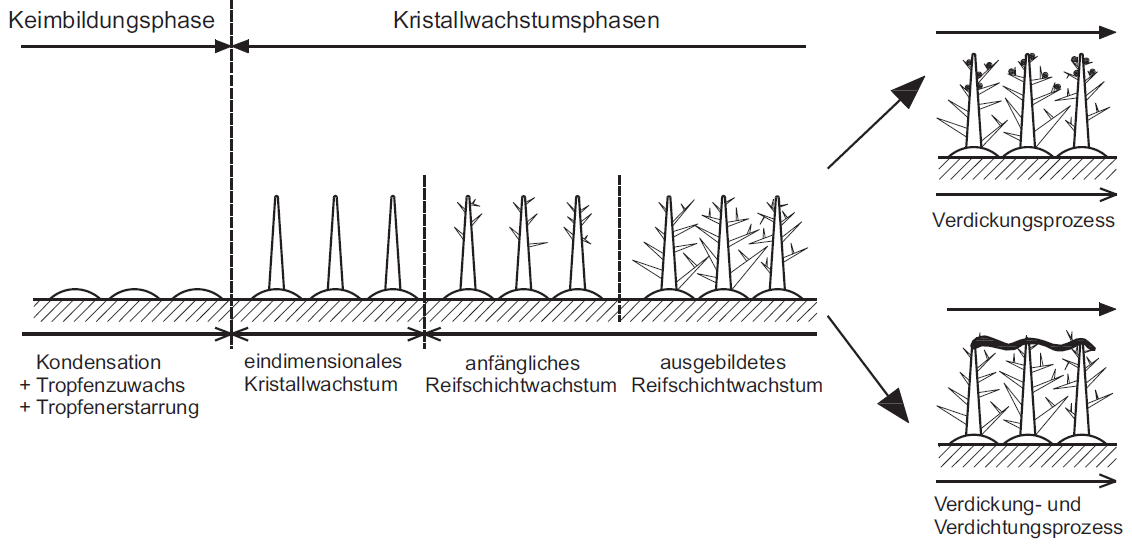
\includegraphics[width=0.85\textwidth]{Pictures/Reifbildungsphasen_Schydlo.png}
\caption{Kristallwachstum auf einer ebenen Oberfläche \citep{Schydlo2010}}
\label{fig:Kristallwachstum}
\end{figure}


In Abbildung \ref{fig:Kristallwachstum} sind die drei Kristallwachstums-Phasen nach \textsc{\citeauthor{Hayashi1977}} sowie die vorhergehende Keimbildungsphase, eingeführt in \citep{Sahinagic2004}, dargestellt. 

\subsubsection*{Keimbildungsphase}

In der Keimbildungsphase bilden sich zunächst Wassertropfen auf der Lamellenoberfläche, die trotz Temperaturen kleiner als der Gefrierpunkt nicht erstarren, sondern zu größeren Tropfen anwachsen. Je kleiner die Unterkühlung, desto größer werden die Tropfen, bevor sie erstarren und in die erste Kristallwachstumsphase übergehen. 

\subsubsection*{Eindimensionales Kristallwachstum}
Die erste Phase ist gekennzeichnet durch Kristallwachstum senkrecht zur Oberfläche und mit einheitlicher Wachstumsgeschwindigkeit. Dies führt aufgrund der sich stetig vermehrenden Kristalle zu einer erhöhten Rauigkeit.  

\subsubsection*{Reifschichtwachstumsphase}
In der zweiten Phase beginnt das dreidimensionale Wachstum. Die Kristalle fangen an sich miteinander zu verästeln. Ein poröses Kristallgitter entsteht. Aufgrund des  Wärmeleitwiderstandes, der mit der Reifdicke steigt, erhöht sich die Oberflächentemperatur der Reifschicht. Des weiteren kommt es zu einem Massenstrom innerhalb der Reifschicht, ausgelöst durch Diffusion. Die Diffusion rührt aus  dem  Konzentrationsunterschieden zwischen der Lamelle und der Reifoberfläche. Der Wassermassenstrom läuft in das poröse Kristallgitter und gefriert dort in Nähe der Lamelle. Die Dichte der Reifschicht steigt und mit ihr der Wärmewiderstand. Dies führt zu einer Erhöhung der Oberflächentemperatur der Reifschicht und schließlich zur Überschreitung des Gefrierpunktes von Eis. Die Spitzen des Kristalle schmelzen und es bildet sich Kondensat. Die dritte Wachstumsphase beginnt. 

\subsubsection*{Vergletscherung}

Das flüssige Wasser läuft aufgrund der Kapillarwirkung der Kristalle in die Zwischenräume des Kristallgitters und gefriert dort wieder. Die Kristallgitter werden dichter und kompakter. Dies führt zur Steigerung der Wärmeleitfähigkeit der Reifschicht. Es wird von einer Vergletscherung gesprochen. Die Oberflächentemperatur der Reifschicht sinkt erneut und fällt erneut unter den Gefrierpunkt. Nun kann die feuchte Luft erneut an der Oberfläche des Reifs desublimieren. Der Prozess wiederholt sich solange, bis das Eis so kompakt ist, dass kein weiteres Kondensat mehr in die Reifschicht eindringen kann. 

\subsection*{Physikalische Eigenschaften von Eiskristallen}

 Im vorangegangenen Abschnitt \ref{subsec:Reifbildung} wurden die einzelnen Bildungsphasen von Eiskristallen beschrieben. In diesem Abschnitt wird auf die Eigenschaften von Eiskristallen eingegangen und dargestellt wie sie sich während eines Vereisungsvorganges eines Luftkühlers verändern. 
 
Gefriert ein Tropfen Wasser und wird zum Eiskristall, so verändern sich die physikalischen Eigenschaften des Tropfens. In der Arbeit von \textsc{\citeauthor{Schydlo2010}} verdeutlichen zunächst zwei Diagramme, abgebildet in \ref{fig:Zeitverlaufe von Reifdichte und -dicke}, wie sich die Reifdicke und die Reifdichte während eines Vereisungsvorgang verändern. 

\begin{figure}
\centering
    \subfigure[Reifdichte]
    {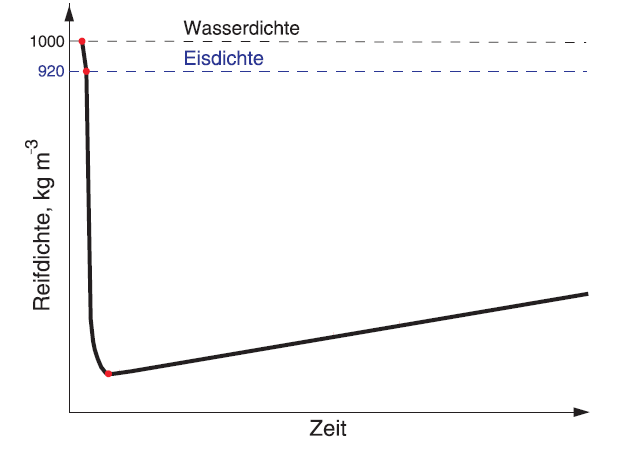
\includegraphics[width=0.50\textwidth]{Pictures/Reifdichte_Schydlo.png}}
    \subfigure[Reifdicke]{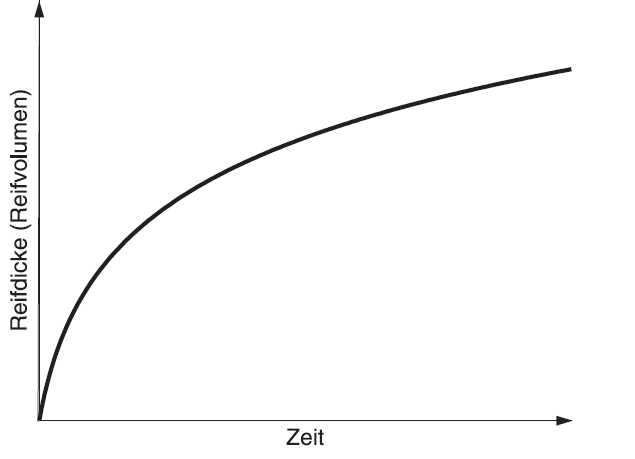
\includegraphics[width=0.48\textwidth]{Pictures/Reifdicke_Schydlo.png}}
\caption{Schematischer Reifdichte- und Reifdickeverläufe beim Vereisungsvorgang eines Tropfen Wassers \cite{Schydlo2010}}
\label{fig:Zeitverlaufe von Reifdichte und -dicke}
\end{figure}

Da Diagramm \ref{fig:Zeitverlaufe von Reifdichte und -dicke}(a) zeigt den Dichteverlauf, aufgetragen über die Vereisungszeit. Die Dichte eines Tropfens fällt beim Gefrieren von 1000 kg/m$^3$ auf 920 kg/m$^3$ sinkt. Danach tritt das in Abschnitt \ref{subsec:Reifbildung} beschriebene eindimensionale Wachstum ein, sodass die Reifdichte bis auf ein Minimum fällt. Danach tritt die dreidimensionale Wachstumsphase und dann die Vergletscherungsphase ein. Die Dichte  steigt jetzt langsam, aber kontinuierlich wieder an.

\begin{figure}[htb]
\centering	
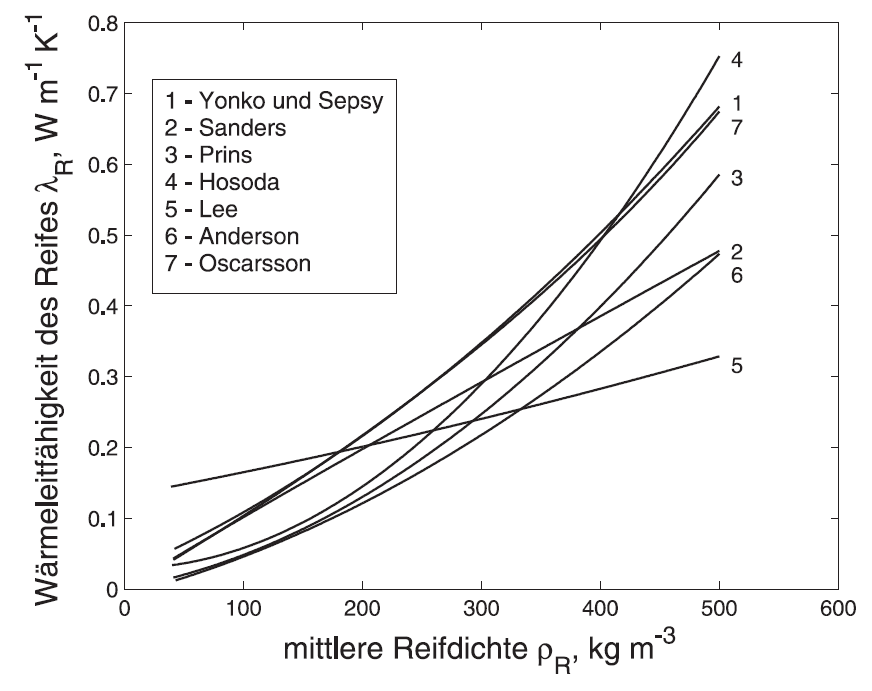
\includegraphics[width=0.55\textwidth]{Pictures/Waermeleitfaehigkeit_Schydlo.png}
\caption{Wärmeleitfähigkeit des Reifs aufgetragen über die mittlere Reifdichte \citep{Schydlo2010}}
\label{fig:Waermeleitfaehigkeit}
\end{figure}

Im \ref{fig:Zeitverlaufe von Reifdichte und -dicke}(b) ist der Reifdickenverlauf aufgetragen. Aus diesem lässt sich entnehmen, dass kurz nach Beginn die zeitliche Änderung der Reifdicke maximal ist. Das heißt, dass der Massenstrom an Kondensat, das sich an der Lamelle absondert und dann gefriert, am Anfang am größten ist und findet während des eindimensionalen Wachstums auf statt. Beim dreidimensionalen Wachstum und späteren Vergletscherung flacht die Kurve ab und strebt gegen einen Sättigungswert. 


 
Mit der Reifdicke verändert sich wiederum die Wärmeleitfähigkeit des Reifes, abgebildet in \ref{fig:Waermeleitfaehigkeit}. In dem Diagramm sind mehrere Berechnungsmodelle aufgetragen, die die Wärmeleitfähigkeit als Funktion der mittleren Reifdichte abbilden. Alle Modelle sagen einen Anstieg von $\lambda$ mit steigender Reifdichte voraus. Dies hängt mit der Verdichtung des Eises während der Vergletscherungsphase zusammen. Die führt dazu, dass Reif mit einer geringen Dichte gleichzeitig als sehr guter Isolator fungiert. \citep{Baehr2013}  \citep{Kosowski2009}





\section{Kältetechnik}
\label{sec:Kaeltetechnik}

Die Kältetechnik wird in verschiedensten Einsatzgebieten eingesetzt, um Kälte zu erzeugen bzw. einem definierten Raum Energie in Form von Wärme zu entziehen. 

Das Konservieren von Lebensmittel ist  der ursprüngliche Hauptzwecke der Kältetechnik und ist auch heute noch aktuell. Bereits 3000 Jahre v. Chr. nutzten die Ägypter und Mesopotamier Natureis, um ihre Nahrungsmittel länger haltbar zu machen.\citep{Danfoss2006}

Im Jahre 1834 meldete der US-Amerikaner Jacob Perkins sein Patent zum Thema Kältetechnik in England an. Das Patent beschreibt eine Kaltdampfmaschine in einem geschlossenen Kreislauf mit dem feuergefährlichen Äthyläther als Kältemittel.\citep{Siemens2007}

Carl von Linde baute nach konstruktiven Verbesserungen der Kaltdampfmaschine und Verwendung von Ammoniak als Kältemittel im Jahre 1876 die erste praxistaugliche Kälteanlage. Die ersten Anlagen wurden durch die Maschinenfabrik Augsburg-Nürnberg gebaut und an Brauereien sowie später auch an die Schifffahrt vertrieben.

Mit steigender Bedeutung von Elektrizität als Energieträger nach dem 1.Weltkrieg nahm auch die Entwicklung und der Bedarf an Kälteanlagen zu. Im Jahre 1920 startet die Firma \textit{General Electric} mit der Serienherstellung von Haushaltkühlschränken mit Hermetik-Verdichtern.

Das vielseitige Gebiet der Kältetechnik umfasst alle Technologien, die zur Bereitstellung von Kälteenergie dienen. Sie unterscheiden sich in der benötigten zuzuführenden Energien, Einsatzbereich und eingesetzten Kältemitteln.  Zu den wichtigsten und heute meist verwendeten Technologien gehören folgende Technologien

\begin{itemize}

\item Kompressions-Kälteprozess: \textit{Prozess wird angetrieben durch Zufuhr mechanischer Energie}
\item Sorptions-Kälteprozess: \textit{Prozess wird angetrieben durch Zufuhr von Wärmeenergie}
\item Linde-Verfahren.

\end{itemize}

Weitere nicht so weitverbreitete Technologien der Kältetechnik, jedoch technisch interessante Verfahren  sind zB. das  \textit{Wirbelrohr},  \textit{Magnetische Kühlung} oder das Kühlen mittels einem Peltier-Element. Diese Verfahren werden meist nur unter hohem Energieverbrauch in Sonderfällen angewandt. \citep{Grote2014}

Da sich diese Masterarbeit mit dem Aufbau eines Prüfstandes zur Untersuchung von Abtaumethoden einer Kompressionskälteanlage beschäftigt, wird in den folgenden Kapitel ausschließlich auf diese Technologie eingegangen. Für weitere Informationen bezüglich der anderen Technologien sei an dieser Stelle auf die Literatur \citep{Baehr2013}, \citep{Grote2014} und \citep{Grote2014} verwiesen.



\subsection{Komponenten eines Kaltdampfprozesses}
\label{subsec:Komponenten eines Kaltdampfprozesses}

Die Komponenten für einen einfachen Kaltdampfprozess  besteht aus vier Komponenten:

\begin{itemize}
\item der Kompressor
\item der Verflüssiger 
\item das Drosselvenil Expansionsventil
\item der Verdampfer. 
\end{itemize}

In Abbildung \ref{fig:einfacher Kältekreislauf} sind die vier Komponenten mit ihren Zustandspunkten dargestellt.

\begin{figure}[htb]
\centering		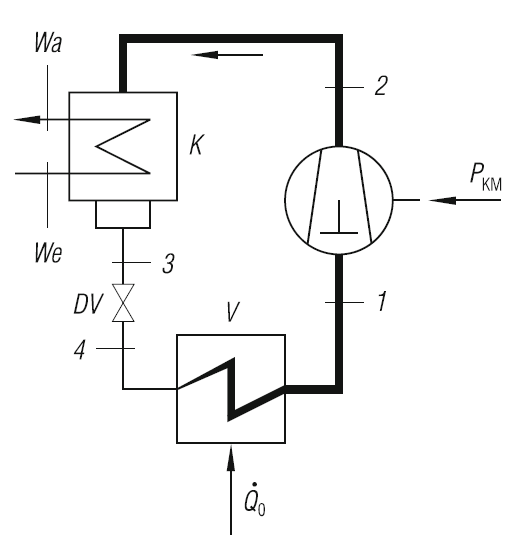
\includegraphics[width=0.50\textwidth]{Pictures/Kaltekreislauf_beahr.png}
\caption{Einfacher Kältekreislauf \citep{Baehr2013}}
\label{fig:einfacher Kältekreislauf}
\end{figure}

\subsubsection*{Der Kompressor}
Der Kompressor bildet das Herzstück der Kälteanlage. Er verdichtet das gasförmige Kältemittel von niedrigem Druck auf ein höheres Druckniveau. Um diese Arbeit zu verrichten, wird der Verdichter mit elektrischer Energie versorgt. Der Kompressor gibt es in verschiedenen Bauvarianten. Die zwei wichtigsten Bauvarianten sind der \textit{Hubkolbenverdichter} und der \textit{Rotationskolbenverdichter}. Die Baugruppen der Verdichter werden in offene, halbhermetische und vollhermetische Verdichter unterschieden. Schrauben-,Scroll- sowie Turboverdichter sind Bauarten der \textit{Rotationskolbenverdichter}. 



Ein wichtiges Kriterium bei Verdichtern ist das Druckverhältnis von Ansaugdruck, vor der Kompression, und dem Ausgangsdruck. Das Druckverhältnis $\pi$ ist definiert als:



\begin{equation}
\pi := \frac{p_{aus}}{p_{ein}}.
\label{Druckverhältnis}
\end{equation}

\subsubsection*{Der Verflüssiger}

Dem Kältemittel wird im Verflüssiger auf einem hohen Druckniveau Wärme entzogen. Der Verflüssiger kühlt das überhitzte, gasförmige Kältemittel ab. Beim Austritt aus dem Verflüssiger ist das Kältemittel meist vollständig kondensiert. 
Um einen Wärmeentzug zu bewerkstelligen gibt es drei Bautypen:

\begin{itemize}
\item Wassergekühlte Verflüssiger
\item Luftgekühlte Verflüssiger
\item Verdunstungsverflüsssiger
\end{itemize}

Wassergekühlte Verflüssiger können, aufgrund der besseren Wäärmeübertragung verglichen zu Luft, sehr kompakt gebaut werden. Eine typische Bauform ist das \textit{Bündelrohrverflüssiger}.
In der Praxis werden am häufigsten luftgekühlte Verflüssiger eingesetzt. Um die gleiche Kühlleistung wie ein wassergekühlter Verflüssiger zu erreichen, werden Lamellen und Ventilatoren eingesetzt. Die Lamellen vergrößern die Fläche für die Wärmeübertragung mit der Luft. Ventilatoren ermöglichen durch einen höheren Luftdurchsatz und der daraus resultierendem höhere Wärmeübertragung eine größere Kühlleistung und eine kompaktere Bauform der Wärmeübertragers. Diese Variante hat den Vorteil, dass die einen wartungsfreien Betrieb  sowie eine einfache Reinigung ermöglicht.


\subsubsection*{Das Expansionsventil}

Das Expansionsventil versorgt den Verdampfer mit dem nötigen Kältemittel-Massenstrom. Die Zuführung des Kältemittels erfolgt über eine Druckdifferenz. Durch eine lokale Verengung des Strömungquerschnitts, verringet sich der Druck des durchfließenden Kältemittels. Das Kältemittel vergrößert sein Volumen und es kommt zur Expansion. Die Druckreduzierung erfolgt ohne zusätzliche Arbeit. Im idealen Fall wird bei diesem Prozess auch keine Wärme abgefuhrt; der Prozess ist \textit{isenthalb}. 
Das Expansionsventil trennt zusammen mit dem Kompressor die zwei Druckseiten des Kältekreislaufes. Es gibt Expansionsventile sowohl als regelbare und nicht regelbare Ausführungen. Bei kleineren Anlagen erfolgt die Expansion ungeregelt zum Beispiel durch Kapillarrohre. Geregelte Expansionsventile werden in mittleren und großen Kälteanlagen eingesetzt. Die Regelung erfolgt durch die Querschnittsänderung und dem damit einhergehendem Druckabfall.  

\subsubsection*{Der Verdampfer}

In dem Verdampfer wird das Kältemittel eingespritzt. Das Kältemittel verdampft und entzieht seiner Umgebung dabei Wärme. Aufgrund der vielfältigen Anforderungen an Verdampfer, gibt es eine Vielzahl an Bauarten für Verdampfer. Mögliche Bauarten sind 

\begin{itemize}
\item Glattrohrverdampfer
\item Beripptes Verdampferregister
\item Rippenrohrverdampfer
\end{itemize}

Um eine möglichst große Kälteleistung zu ermöglichen, werden wie beim Verflüssiger auch, Ventilatoren eingesetzt. Die Ventilatoren erzwingen einen Luftstrom durch den Verdampfer und erhöhen damit die Wärmeübertragung zwischen der Luft und den Verdampferrohren. 

%\newpage
\subsection{Abtaumethoden}
\label{subsec: Abtaumethoden}

Um einen vereisten Luftkühler abzutauen, gibt es mehrere Methoden. Die Methoden unterscheiden sich in der Installation, Schnelligkeit, Effizienz und Effektivität. Je nach Einsatzbereich und Anlage wird entschieden welche Abtaumethode installiert und eingesetzt wird. Mehrkosten für die Installation sowie weitere Betriebskosten sind bei der Entscheidung stets ein nicht zu vernachlässigender Punkt.
Die in der Praxis am weit verbreitesten Methoden sind  die \textit{Heißgas-Abtauung}, \textit{Prozessumkehrung}, \textit{elektrische Abtauung} und \textit{Umluft-Abtauung}.

Die Tabelle \ref{tab:Vor- und Nachteile} gibt einen Überblick über die Vor- und Nachteile der jeweiligen Abtaumethode. 

\subsubsection*{Heißgas-Abtauung}

Die Heißgasabtaung wird durchgeführt indem das Heißgas aus dem Kompressor anstatt in den Verflüssiger direkt in den vereisten Verdampfer leitet. Für diese Methode wird eine Bypass-Leitung von dem Austritt vom Verdichter bis zum Eingang des Expansionsventil gelegt. Mittels zwei Drei-Wegeventilen kann diese Leitung geöffnet bzw. geschlossen werden. In der Abtauphase ist der Verflüssiger vom Kreislauf ausgeschlossen, damit kein flüssiges Kältemittel in den Verdampfer fließt. \citep{Baehr2013}
Der Prozess läuft in 3 Schritten ab:

\begin{itemize}
\item[1$\longrightarrow$ 2] Kältemittel-Verdichtung durch den Kompressor unter Aufnahme elektrischer Energie

\item[2 $\longrightarrow$ 3] Isenthalpe Entspannung durch das Expansionsventil

\item[3 $\longrightarrow$ 1] Wärmeabgabe an Rohre, Lamellen und das Eis. 
\end{itemize}


In Abbildung \ref{fig:Heissgas-Abtauung} ist der rechtsläufige Kreisprozess in einem ln p, h- Diagramm für das Kältemittel R290 abgebildet. 


\begin{figure}[htb]
\centering
\subfigure[Fließbild. Links: Kühlbetrieb, Rechts: Abtaubetrieb]
{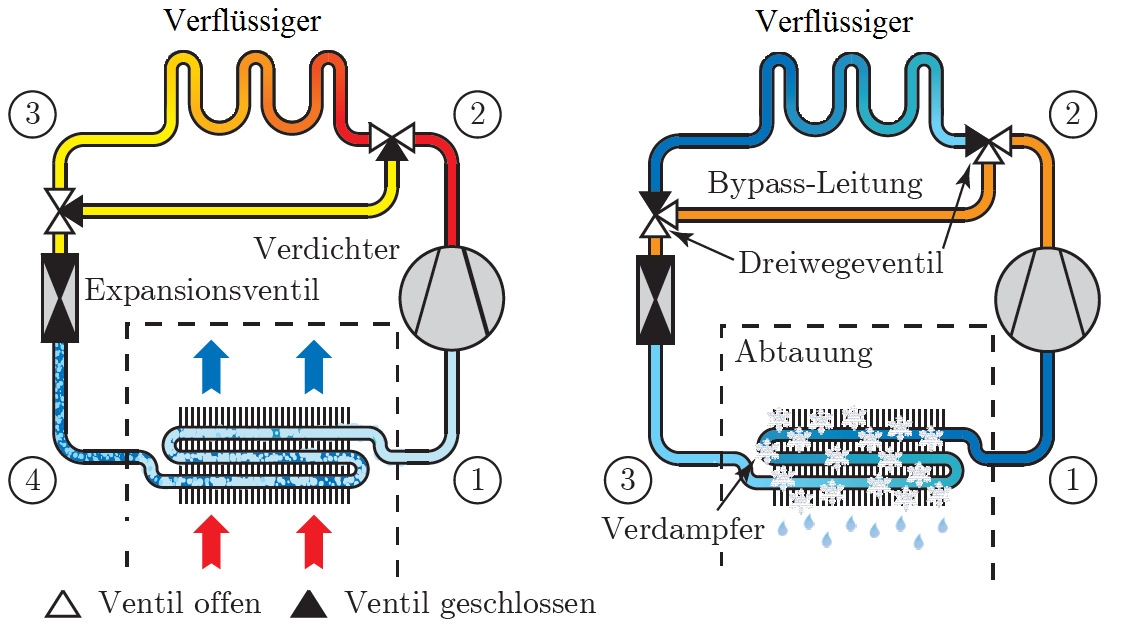
\includegraphics[width=0.640\textwidth]{Pictures/HeissgasKosowski.png}}
\subfigure[Zustandspunkte im ln p,h Diagramm]{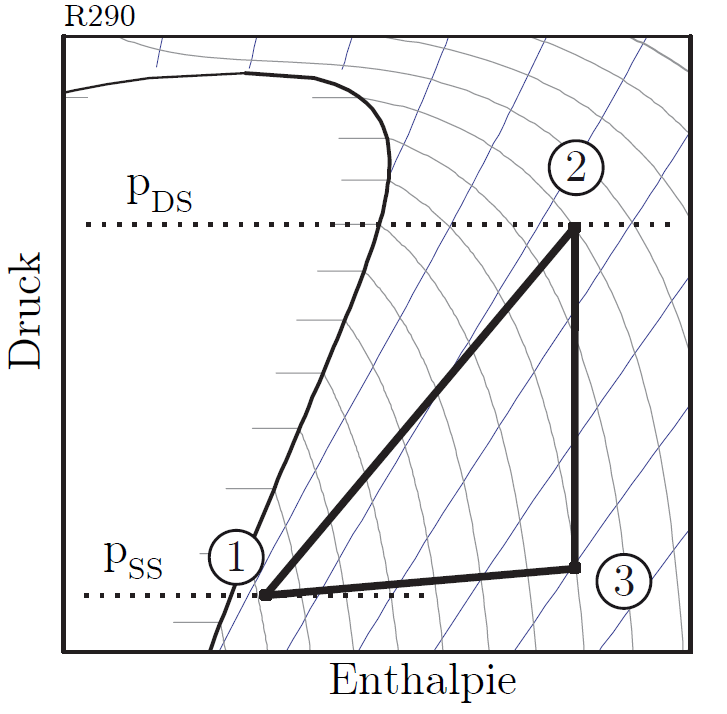
\includegraphics[width=0.35\textwidth]{Pictures/HeissgasEnthalpieDiagrammKosowski.png}}
\caption{Heißgas-Abtauung \citep{Kosowski2009}}
\label{fig:Heissgas-Abtauung}
\end{figure}



\subsubsection*{Prozessumkehrung}

Bei der Abtauung durch Prozessumkehrung wird die Funktion der Wärmeübertrager vertauscht. Während des Abtauprozesses fungiert der Verdampfer als Verflüssiger und der Verflüssiger hat die Aufgabe des Verdampfers inne. Die Prozessumkehrung wird in der Regel durch ein Vierwegeventil gewährleistet. Das Vierwegeventil wird bei der Abtauung geschaltet und leitet das Kältemittel nach dem Kompressor erst in den vereisten Verdampfer. Das überhitzte Kältemittel durchströmt den Verdampfer auf hohem Druckniveau und gibt Wärme an die Rohre und Lamellen des Luftkühlers sowie an das Eis ab.

Die Versuchsalage, die in dieser Arbeit optimiert worden ist, ist mit dieser Technologie ausgestattet. Der Umkehrprozess wird näher im Kapitel \ref{cha: Versuchsaufbau} erläutert. 


\begin{figure}[htb]
\centering		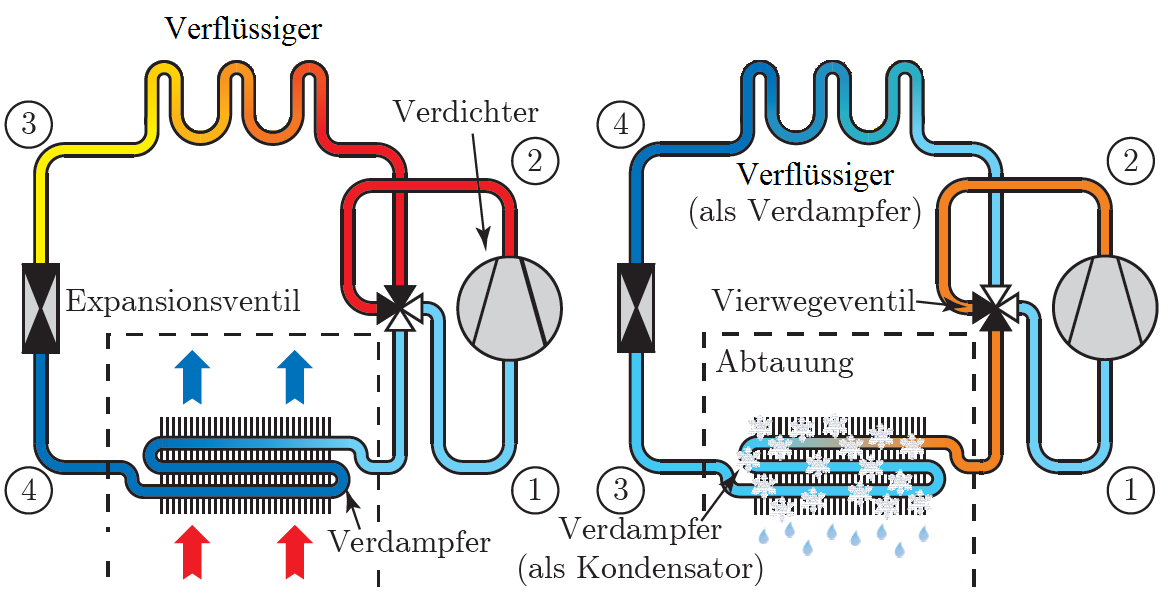
\includegraphics[width=0.7\textwidth]{Pictures/Prozessumkehrung_Kosowski.png}
\caption{Links: Kühlbetrieb. Rechts:Heißgas-Abtauung \citep{Kosowski2009}}
\label{fig:Prozessumkehrung}
\end{figure}

\subsubsection*{Elektrische Abtauung}

Eine weitere Möglichkeit der Abtauung ist die elektrische Abtauung. Bei dieser Methode sind Widerstandsheizungselemente in den Wärmeübertrager des Verdampfers installiert. Die Widerstandsheizung wandelt elektrische Energie in thermische Energie um, und überträgt diese weiter an den Wärmeübertrager und das Eis. 

Das Prinzip der Widerstandsheizung beruht auf einen niedrig ohmigen Widerstand, der von Strom durchflossen wird und sich dabei erhitzt. Die Widerstandsheizung, auch Heizpatronen genannt, können in Reihe oder auch parallel geschaltet werden. Bei der Erhitzung  Die abfallende elektrische Spannung über einen Heizswiderstand errechnet sich nach dem Ohmischen-Gesetz zu :

\begin{equation}
U = R I
\label{eq: Ohmisches Gesetz}
\end{equation}

Hierbei ist $R$ der spezifsche Widerstand des eingesetzen Material, meistens Metalle,  und $I$ die angelegte Stromstärke. Ein Heizwiderstand hat einen Wirkungsgrad von 100 $\%$ und wandelt somit die komplette elektrische Leistung in thermische um:

\begin{equation}
\dot{Q}_{th}= P_{el }= U I = \frac{U^2}{R} =  R I^2 
\label{eq:Leistung Heizwiderstand}
\end{equation}

Die thermische Leistung ist folglich proportional zu der angelegten Spannung $U$. Die Widerstände sind über die Spannung $U$ regelbar. Der Wärmeübergang von den Heizpatronen auf den Wärmeübertrager ist entscheidend für ein effizientes Abtausystem. Je formschlüssiger die Heizpatronen in den Verdampfer installiert sind, desto besser der Wärmeübergang und effizienter die Abtauuung.  
Die Versuchsanlage dieser Arbeit ist auch mit dieser Abtautechnologie ausgestattet. 

\subsubsection*{Umluft-Abtauung}

Die Umluft-Abtauung ist eine weitere in der Praxis häufig verwendete Abtaumethode. Hierbei wird der Verdampfer durch die vorbeiströmende Umluft abgetaut. Um dies zu ermöglichen muss zum einen der Ventilator in der Abtauphase laufen und zum anderen die Umgebungstemperatur größer als 0 $°$C sein. Ein Vorteil dieses Verfahrens ist, dass die Wärmeübertragung luftseitig geschieht und dadurch die zuzuführende Wärme nicht zusätzlich das Material des Verdampfers erhitzen muss. 

Diese Abtaumethode wird in der Arbeit nicht näher untersucht. Deswegen wird an dieser Stelle auf die  Literaturquellen \citep{Breidenbach2014} und \citep{Ehrbar2002} verwiesen. 

%\subsubsection{Gegenüberstellung der Abtaumethoden}
%\label{subsubsec:Gegenüberstellung }



%\begin{landscape}

\begin{table}%[htb]
\centering
\caption{Vor- und Nachteile der verschiedenen Abtaumethoden   	\citep{Breidenbach2014}, \citep{Refrigeration2000}, \citep{Yin2012}, \citep{Huang20091697}
} \vspace{6pt}

\label{fig:PCM_Slurry1}
%\begin{tabular}{p{3.9cm}p{8cm}p{8cm}lll} 
\begin{tabular}{p{3.8cm}p{5.6cm}p{5.6cm}lll}
\hline
\textbf{Abtaumethode} &\textbf{Vorteile} & \textbf{Nachteile}\\
\hline
\hline

\textbf{Heißgas-Abtauung} 
&
$\bullet$ Guter Wärmeübergang zwischen Heißgas,Rohre und Eis
\newline								  			
$\bullet$ Unkomplizierte Wartung
\newline			  
$\bullet$ Kurze Abtaudauer		
\newline			
$\bullet$ Schnelles Wiederanfahren möglich	

&$\bullet$ Höherer Planungs- und Installationsaufwand  
\newline
$\bullet$ Zusätzliche Kühlung des Kompressors in Abtauphase ist erforderlich 
\newline 
$\bullet$ Höhere Druckverluste durch zusätzliche Komponenten 
\newline
$\bullet$ kritische Kältemittel-Menge bestimmt durch Abtauleistung \\  
   
\hline
\textbf{Prozessumkehrung}
&$\bullet$ Guter Wärmeübergang zwischen Heißgas,Rohre und Eis  													
\newline								
$\bullet$ Unkomplizierte Wartung
\newline	
$\bullet$ Kurze Abtaudauer		
\newline			 
$\bullet$ geeignet für Verbund-Systeme		
&$\bullet$ Abtropfwanne ist nicht beheizt   
\newline
$\bullet$ Höherer Planungs- und Installationsaufwand
\newline
$\bullet$ Nicht nachrüstbar
\newline
$\bullet$ Höhere Druckverluste durch zusätzliche Komponenten								
\newline
$\bullet$ Kritische Kältemittel-Menge bestimmt durch Abtauleistung\\


\hline
\textbf{Elektrische Abtauung }
&$\bullet$ Einfache Komponenten und Installation 
\newline 
$\bullet$ \textit{Stand-Alone}-System ist nachrüstbar		
\newline
$\bullet$ Hohe Regelgenauigkeit	
\newline
$\bullet$ Abtropfwanne ist beheizbar 					
&
$\bullet$ Schlechter Wärmeübergang 
\newline					
$\bullet$ Verursacht Kältemittelbewegung in den Sammler
\newline 
$\bullet$ Brandgefahr im Falle von Kabelbruch  
\newline
$\bullet$ Zeitliche Verzögerung beim Abtauprozess 
\newline
$\bullet$ Hohe thermische Belastung der Komponenten    
\\

 
\hline
\textbf{Umluft-Abtauung }
&
$\bullet$	Keine zusätzlichen Komponenten nötig			 
\newline
$\bullet$	Günstig										
\newline
$\bullet$	Keine zusätzlicher Wärmeeintrag ins System	  
\newline
$\bullet$	Keine Abtauung der Abtauwanne möglich	
&
$\bullet$ Bei überdimensionierten Kompressoren sehr hohe Abtaudauer möglich
\newline
$\bullet$ Funktioniert nur mit Umgebungstemperaturen über $ 2\,^{\circ}\mathrm{C} $
\\
\hline

\end{tabular}
\label{tab:Vor- und Nachteile}
\end{table}
%\end{landscape}


\newpage
\section{Federn}
\label{sec:Federn}

Der Einsatzbereich von Federn ist genau so vielfältig wie die verschiedenen Bautypen, Größen und Werkstoffen. Je nach Funktion können Feder können zug-,druck-, torsion- oder biegebeansprucht werden. 
Die Hauptfunktionen umfassen die Gewährleistung des Kraftflusses und der Kraftverteilung, Speicherung von Energie, Ausdehnungsausgleich, Dampfungssysteme oder Schwingungssysteme. 
Federn werden charakterisiert durch ihre Feder-Kraft-Kennlinie bzw. Moment-Verdrehwinkel-Kennlinie. 

In dieser Arbeit wurde eine rechteckige Blattfeder dimensioniert, gefertigt und als Teil eines Wägesystems kalibriert, siehe Abschnitt \ref{sec:Waegesystem}. Deshalb werden in diesem Abschnitt nur auf biegebeanspruchte, rechteckige Blattfedern näher eingegangen. 

\begin{figure}[htb]
\centering
\subfigure[Rechteckblattfeder (Ansicht und Draufsicht)]
{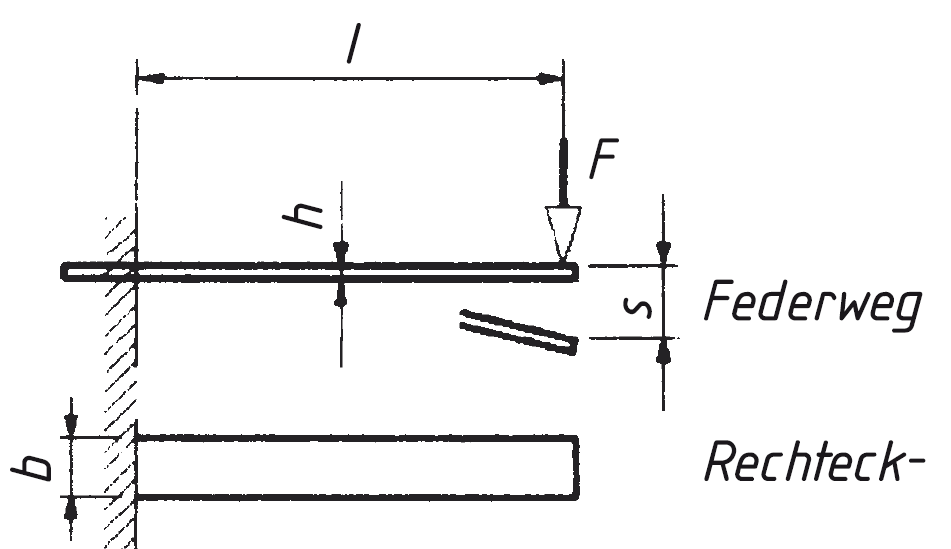
\includegraphics[width=0.4\textwidth]
{Pictures/Federprinzip.png}}
\subfigure[Kraft-Weg-Kennlinien]{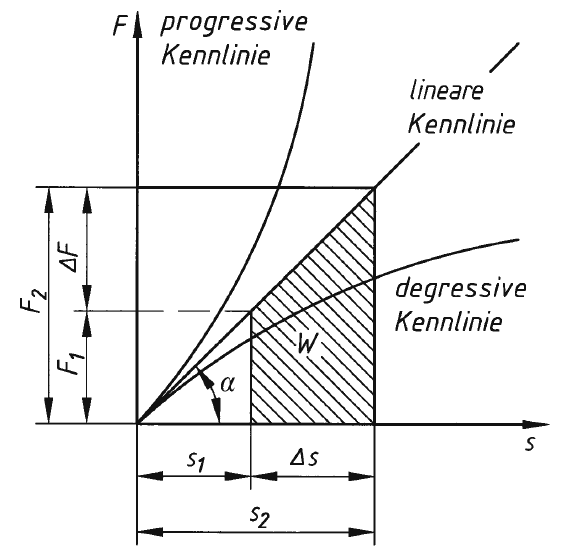
\includegraphics[width=0.4\textwidth]
{Pictures/Kraft-Weg-Kennlinie.png}}
\caption{Blattfeder und Feder-Kennlinien \citep{Wittel2011}}
\label{fig:Federdiagramm}
\end{figure}

Die Abbildung \ref{fig:Federdiagramm}(a) zeigt das Prinzip einer einsetig eingespannten, rechteckigen Blattfeder und \ref{fig:Federdiagramm}(b) drei unterschiedliche Kraft-Weg-Kennlinien. $l$ ist die Länge von der Einspannung bis zum Angriffspunkt der Kraft $F$. $h$ ist die Höhe und $b$ die Breite der Feder. Der Federweg $s$ resultiert aus der Verformung der Feder durch die Belastung mit der der Kraft $F$.

Eine rechteckige Blattfeder verhält sich bei Zunahme der belastenden Kraft $F$ , wie die $lineare~Kennlinie$ im Diagramm aufzeigt. Die Kraft $F$ und der Federweg $s$ sind zu einander proportional. Eine Verdoppelung der Kraft zieht gleichzeitig eine Verdoppelung des Federweges nach sich. Die meisten eingebauten Federn verfügen über eine solche lineare Kennlinie. 

Die aufgenommene Arbeit $W$ ist die Arbeit einer mit $F_1$ vorgespannten Feder, die zusätzlich zu $F_1$ mit $\Delta F$ belastet wird. Die gesamte Kraft beträgt $F_2 = F_1 + \Delta F$. Durch die zusätzliche Kraft verbiegt sich die Feder um $\Delta s$ von $s_1$ auf $s_2$. Die aufgenommene Arbeit $W$ und in Abbildung \ref{fig:Federdiagramm}(b) markierte Fläche errechnet sich zu :

\begin{equation}
W = \frac{1}{2} (F_1 + F_2) \Delta s.
\label{Federarbeit}
\end{equation}


Die Federrate $R$ ist das Verhältnis von der belastender Kraft $F$ zum Federweg $s$:

\begin{equation}
R = tan (\alpha)= \frac{\Delta F}{\Delta s}
\label{eq:Federrate}
\end{equation}


Wie Abbildung \ref{fig:Federrate} zeigt, haben harte Federn eine höhere Federrate. Weiche Feder besitzen hingegen eine kleinere Federrate. 


\begin{figure}[htb]
\centering
\subfigure[Federrate $R$ \citep{Ettemeyer2007}]
{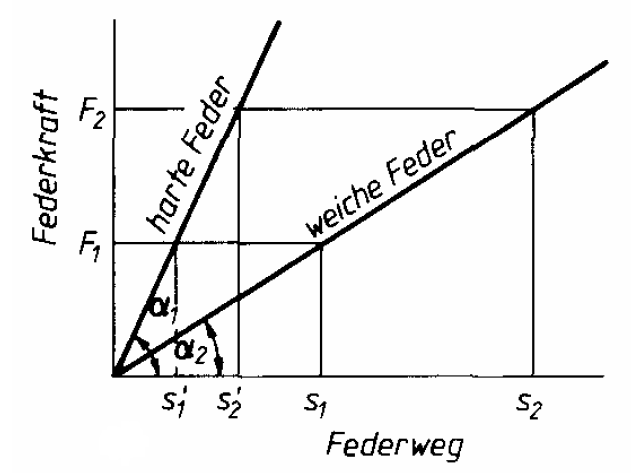
\includegraphics[width=0.52\textwidth]
{Pictures/Federrate.png}}
\subfigure[Federungsarbeit mit Reibungs-Hysterese\citep{Wittel2011}]
{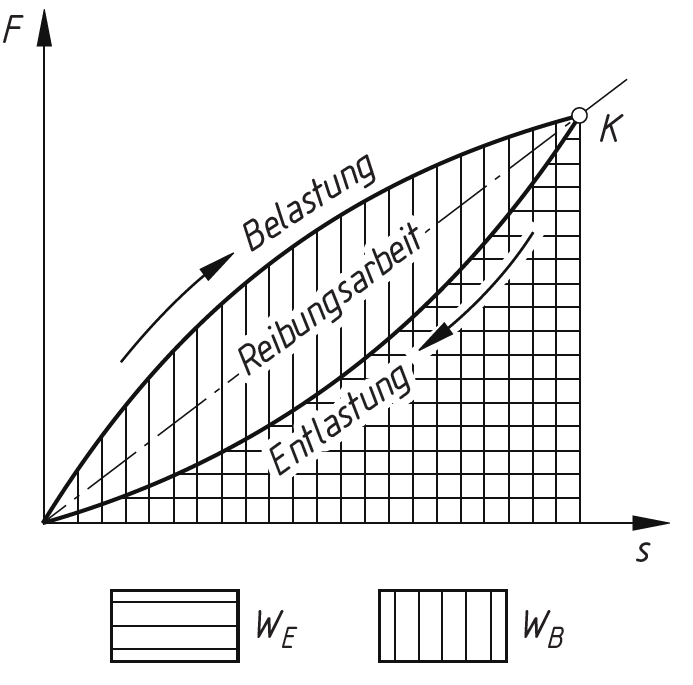
\includegraphics[width=0.4\textwidth]
{Pictures/Federwirkungsgrad.png}}
\caption{Federrate und -wirkungsgrad}
\label{fig:Federrate und -wirkungsgrad}
\end{figure}


Die Biegespannung $\sigma_b$ ist das Verhältnis von der Feder aufzunehmendes Biegemoment $M$ zum Widerstandsmoment $W$. Die Formel für die Biegespannung lautet:

\begin{equation}
\sigma_b = \frac{M}{W}= \frac{6 F l}{b h^2}.
\label{eq:Biegespannung}
\end{equation}

Für rechteckige Blattfeder ergibt sich für den Federweg $s$ am Ende der Feder zu: 

\begin{equation}
s = 4 \frac{l^3}{b h^3} \frac{F}{E}.
\label{eq:Federweg}
\end{equation}

Hierbei ist $E$ das Elastizitätsmodul des verwendeten Werkstoffes. 

Der Federwirkungsgrad jeder realen Feder ist kleiner als 1. Innere und äußere Reibung führen dazu, dass die zur Belastung aufzuwendende Arbeit $W_B$ größer ist als die Arbeit zur Entlastung $W_E$ der Feder, siehe Abbild \ref{fig:Federrate und -wirkungsgrad}(b). Die Formel für $\eta_F$ lautet:

\begin{equation}
\eta_F = \frac{W_E}{W_B}.
\label{eq:}
\end{equation}

Die Auslegung für die verwendete Feder erfolgt im Abschnitt \ref{sec:Waegesystem}. Für weitere Literatur zum Thema Federn wird auf die Litatur \citep{Wittel2011} und \citep{Ettemeyer2007} verwiesen. 


\section{Signalverarbeitung}
\label{sec: Modbus RTU}

\subsection{RS485}
\label{subsec:RS485}

Modbus RTU ist ein Kommunikationsprotokoll, das entweder über RS485, RS232 oder Ethernet kommuniziert. Modbus RTU ist, wie viele andere Feldbusse, nach der Norm IEC 61158 \footnote{\textit{Digital data communication for measurement and control - Fieldbus for use in industrial control systems}} weltweit standardisiert.

Die Vorteile von Feldbussen sind der geringe Verkabelungsaufwand und die Möglichkeit der Eigendiagnose durch das System selbst. Ein Feldbus-System bietet eine hohe Flexibilität gegenüber Erweiterungen oder Änderung des Netzwerkes. Eine Festlegung auf Messbereiche der Sensoren ist nicht notwendig. Ein weiterer Vorteil ist die Möglichkeit der Abfrage unterschiedlicher Messwerte, wie zum Beispiel Temperatur und Druck, von einem Sensor. Die hohe Zuverlässigkeit und hohe Kompatibilität von verschiedenen Sensortypen ist ein weiterer großer Vorteil.

Die Nachteile eines Feldbusses sind die komplexeren Netzwerkstrukturen und -abläufe. Für eine erfolgreiche Implementierung eines Feldbus-Systems wird ein höher qualifiziertes Personal benötigt. Des Weiteren erfordert eine Abfrage der Sensoren meist eine größere Reaktionszeit. Sensoren mit  entsprechender Feldbustechnik sind häufig teurer als Sensoren, die mit analoger Datenübertragung ausgestattet sind. Eine Beschädigung des Kabels kann in manchen Fällen zum Ausfall des kompletten Feldbusses und dessen Sensoren führen. Redundante Netzwerke sind folglich wünschenswert, jedoch nicht immer umsetzbar. 

\begin{figure}[htb]
 \centering		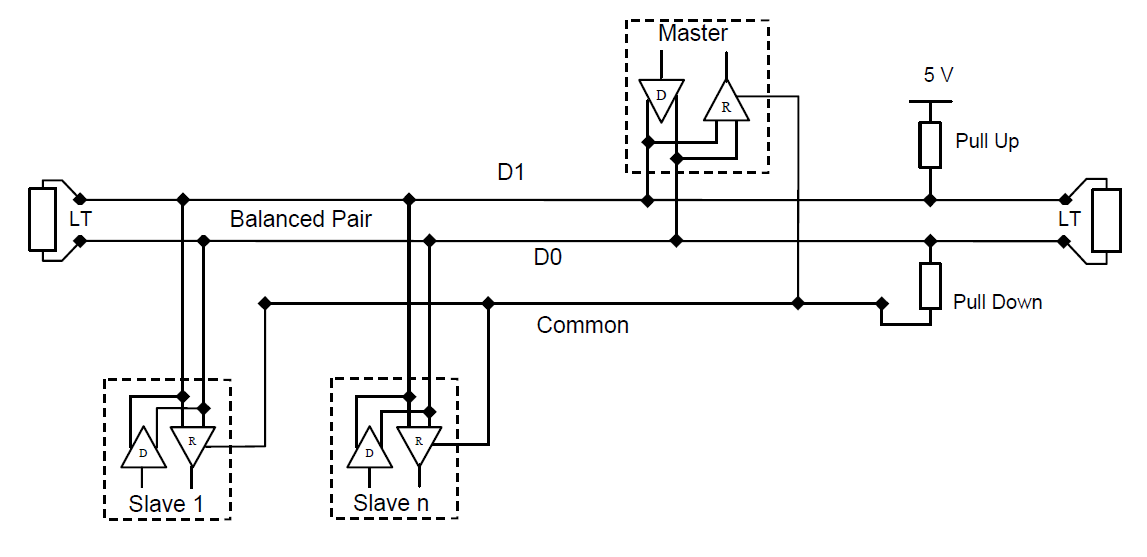
\includegraphics[width=0.94\textwidth]{Pictures/TopologieModbus.png}
 \caption{Zwei-Kabel-Topologie eines Modbus RTU-Feldbusses \citep{MODBUS.ORG2002}  }
 \label{fig:ZweiKabelModbus}
 \end{figure} 
 
Für den Modbus RTU wird nach \citep{MODBUS.ORG2002} eine Serienschaltung der Hardware-Komponenten (engl. \textit{Daisy Chain}) empfohlen. Die Komponenten sind in dieser Topologie in einer Kette verbunden. Ein Netzwerk besteht zu jeder Zeit aus einem Master und multiplen Slaves. Zunächst schickt der Master einen Befehl an einen Slave. Der Slave setzt den Befehl um und schickt dem Master seine Antwort. Die Befehle über die Sendekabel werden nur vom Master empfangen. Die Befehle über das Empfängerkabel werden hingegen nur von den Slaves empfangen.
 
Ein Modbus RTU kann über ein Vier- oder Zwei-Kabel-Topologie verfügen. Ein Vier-Kabel-Topologie verfügt über zwei paarweise Kabel, über die entweder gesendet oder empfangen wird. Die Kabel tragen nach der \textit{EIA/TIA-485 Standard} die Namen $D0$ und $D1$ und werden auch positive und negative \textit{Polarität} genannt. In beiden Topologiefällen können bis zu 32 Slaves angeschlossen werden und bis auf eine Entfernung von größer 1000 m betrieben werden. 

Zusätzlich zu den vier bzw. zwei Kabeln wird ein weiteres Kabel, das \textit{Common}, benötigt. Es stellt ein gleiches Spannungsniveau für alle Slaves sicher. Elektromagnetische Störungen beeinflussen die Datenleitungen ($D0$ und $D1$) und das $Common$-Kabel im gleichen Maße. Die Potentialdifferenz von D1 und D0 zu Common ist folglich konstant. Serielle Bits (0 oder 1) werden mittels Potentialdifferenzen zwischen $D0$ und $D1$ gesendet. Diese Verkabelungsart ist sehr unanfällig gegenüber elektromagnetischen Störsignalen. 

Abbildung \ref{fig:ZweiKabelModbus} zeigt eine typische Zwei-Kabel-Topologie mit Abschlusswiderständen (engl. \textit{Line-Termination} (LT)), einem \textit{Pull-up}- und \textit{Pull-Down}-Widerstand.  Abschlusswiderstände (meist \mbox{150 $\Omega$}, 0,5 W) werden an den zwei Enden der Linientopologie vorgesehen und dienen zur Reduzierung von Signalreflexionen am Ende der Leitungen. Diese können zu Fehlern in der Kommunikation führen. 
Es wird ein \textit{Pull-Up} und ein \textit{Pull-Down} mittels Widerstand zwischen 450 und 650 Ohm durchgeführt. Ein \textit{Pull-Up} zieht die $D1$-Datenleitung auf ein Ruhepotential von 5 V und ein \textit{Pull-Down} die $D0$-Datenleitung auf das Ruhepotential des \textit{Common}-Leiters (meist 0 V).

Das Bussystem RS485 erlaubt es bis zu 32 Sensoren auf einer Entfernung von theoretisch 1000 m anzuschließen.

\newpage 
\subsection{Modbus RTU}
\label{subsec:Modbus-RTU}

Der Modbus RTU basiert auf einer Master-Slaves-Architektur. Ein Master kann mittels eines Befehls an den Slave Informationen schicken, worauf der Slave mit einer Antwort den Befehl ausführt, die Informationen verarbeitet und die erfragten Daten an den Master zurückschickt.

%Um den Ablauf des Programm-Codes des installierten Modbus-Systems zu verstehen, wird zunächst die Befehls- und Datenstruktur erklärt. Dann wird ein Überblick über die Abfrage- bzw. Schreibbefehle gegeben. Zum Schluss wird ein Blick auf den Programmablauf geworfen.

\subsubsection*{Datenstruktur und Timing}

Eine Modbus RTU-Nachricht besteht aus mehreren seriell Bytes (8 Bits). Jedem gesendeten Byte geht ein zusätzliches Stop-Bit voraus. Nach dem Byte gibt es mehrere Möglichkeiten, um das gesendete Byte zu beenden. Die meist genutzten Varianten ist zunächst ein Paritätsbit und ein Stopbit oder zwei Stopbits. 
Das Startbit, auch steigende Flanke genannt,  gibt dem Slave das Signal, dass ein Byte kommt. Der Receiver des Slave wird aktiviert. Dann wird das Byte gelesen. Nach dem Byte kommen nun entweder zwei Stopbits oder ein Paritätsbit und ein Stopbit. Beide Arten signalisierten dem Slave-Receiver, dass der Byte zu Ende ist. 

%Wird mit einem Paritätsbit gearbeitet, kann der Slave-Receive kontrollieren, ob die empfangenen acht Bits des Bytes korrekt sind. Es gibt zwei Paritätsarten: \textit{gerade} und \textit{ungerade}. Wird die \textit{gerade} Paritätsart verwendet, so wird das Paritätsbit 1, wenn das Byte eine gerade Anzahl an Einsen hat. Ein Byte bestehend aus "0000 1111" würde das Paritätsbit auf "1" gesetzt; bei "0001 1111" wäre es "0". Die \textit{ungerade} Parität funktioniert nach dem gleichen Prinzip, nur dass das Pariätsbit "1" ist bei einer ungraden Anzahl "1" im gesendeten Byte. Die Hersteller als auch die \textsc{\citeauthor{MODBUS.ORG2002}} empfehlen die Verwendung einer Parität. Mit Startbit, Paritätsbit und Stopbit ist die Bit-Sequenz 11 Bits lang. 

%Wird keine Parität verwendet, so wird anstatt des Paritätsbits ein weiteres Stopbit verwendet, um die Bit-Sequenz wieder 11 Bits lang zu machen. 


Alle Slaves und der Master müssen in einem Netzwerk die gleichen Einstellungen besitzen. Abweichende Einstellungen führen zu Kommunikationsfehlern. Eine weitere wichtige Eigenschaft eines Modbus-System ist die sogenannte \textit{Baudrate}, ihre Einheit ist bps (\textit{bauds per second}). Sie gibt die Geschwindigkeit der Datenübertragung an. Die diskreten Werte für die Geschwindigkeit können zwischen 1200\dots 115200 bps liegen. 


Eine komplette Modbus RTU-Nachricht besteht aus einer Adresse, einer Funktion, Daten und einer \textit{Cyclical Redundancy Checking} (CRC)-Checksumme. Hier steht die Adresse des Slaves im Netzwerk für den der Befehl gilt. Die Adresse darf im Bereich 1\dots 247 liegen.
Danach kommt die Modbus-Funktion. Es können nicht zwei Befehle simultan ausgeführt werden. Für zwei verschiedene Befehle müssen zwei Nachrichten geschickt werden. 
Dann folgen die Datenbytes. Diese bestehen aus mehreren aneinander gereihten Bytes. In einer Nachricht können 0\dots 252 Datenbytes enthalten sein. 
Am Ende jeder Nachricht findet ein CRC-Test statt. Dieser Test kontrolliert die ganze Modbus-Nachricht auf Fehler, unabhängig von den Paritätseinstellungen.
Vor und nach jeder Nachricht gibt es eine von der Baudrate abhängigenes Timeout. Das Timeout verhindert eine zu hohe CPU-Auslastung auf der Masterseite.\citep{MODBUS.ORG2002} \citep{Schleicher2005}


\begin{figure}[htb]
\centering		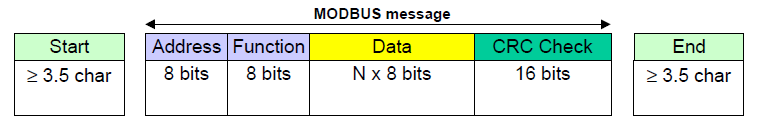
\includegraphics[width=0.90\textwidth]{Pictures/Versuchsaufbau/Modbus_Frame.png}
\caption{Aufbau und Timing einer Modbus RTU-Nachricht \citep{MODBUS.ORG2002}}
\label{fig:}
\end{figure}

\subsubsection*{Befehlsstruktur und Register-Adressen}

Jeder Modbus-Slave hat Informationen oder schreibt Messdaten in seinen internen Speicher. Mögliche Registerspeicher und alle Modbus RTU-Befehle sind im Anhang \ref{Anhang:Modbus} aufgelistet.
Jede Information besitzt eine eindeutige Adresse und hat Lese- bzw. Schreibrechte einprogrammiert.

 Möchte ein Master nun eine Information aus einem Zwischenspeicher lesen oder schreiben bzw. überschreiben, so benötigt er die passende Adresse und für den Zwischenspeicher passenden Befehlstyp.

In der Abbildung \ref{fig:ModbusNachrichtBeispiel} ist beispielhaft eine Druckabfrage eines Drucktransmitters abgebildet. Das Druckwert-Register besteht aus 4 Datenbytes, die zunächst in einen 32 Bit-String und dann in eine REAL-Zahl umgewandelt werden kann. 
Die Anfrage enthält die Startregister-Nummer und die Anzahl der abzufragenden Register. 
Der Slave antwortet auf den Befehl  mit seiner Adresse, den Befehlstyp, die Anzahl der folgenden Datenbytes und mit den Datenbytes selber. Danach erfolgt ein CRC-Test. In grün eingezeichnet sind die Datenbytes und der entsprechende REAL-Zahlenwert. 

\begin{figure}[htb]
\centering		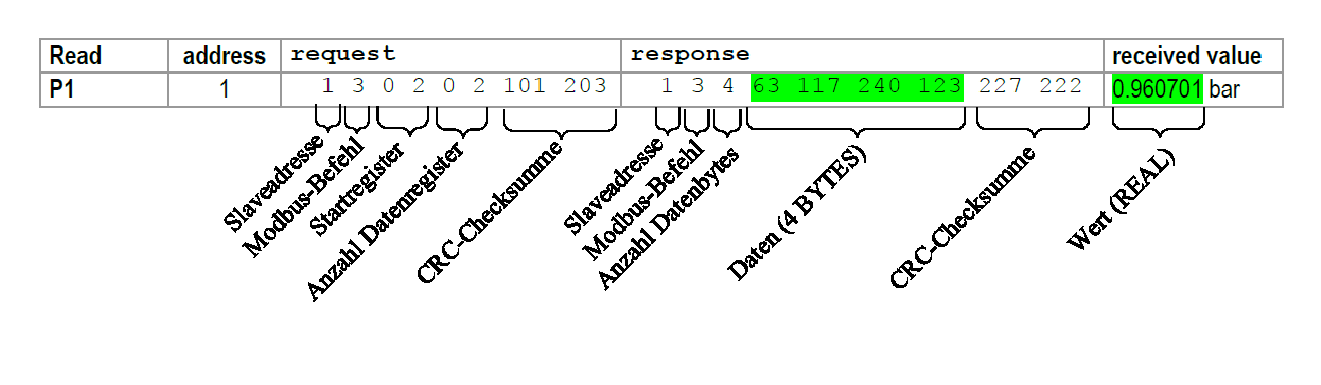
\includegraphics[width=1.0\textwidth]{Pictures/Versuchsaufbau/ModbusBefehlBeispiel.pdf}
\caption{Modbus-Nachrichten Beispiel: Druckabfrage vom Kanal $P1$. Links der Modbusbefehl (\textit{request}) vom Master und rechts die Antwort (\textit{response})}
\label{fig:ModbusNachrichtBeispiel}
\end{figure}






\section{Informationstechnik}


\subsection*{TwinCAT 3}
\label{subsec:TwinCat}

\begin{figure}[htb]
\centering		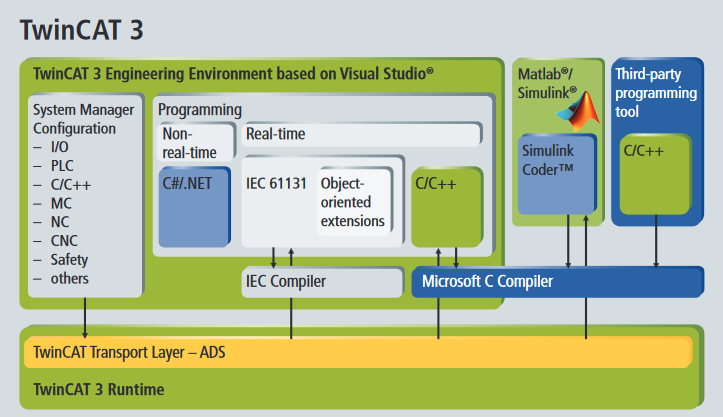
\includegraphics[width=0.90\textwidth]{Pictures/TwinCat3_Beckhoff.png}
\caption{TwinCAT 3 \citep{Beckhoff2016}}
\label{fig:TwinCAT}
\end{figure}


Die im vorherigen Abschnitt vorgestellte Statusmaschine soll mittels einer SPS-Programmierung umgesetzt werden. Zur informationstechnischen Umsetzung wurde die Automatisierungssoftware TwinCAT 3 der Fa. Beckhoff verwendet. TwinCAT ist die Abkürzung von \textit{The Windows Control and Automation Technology} und  ist in die Entwicklungssoftware \textbf{Visual Studio} der Fa.  von Microsoft integriert. Über das Visual Studios wird der Programmcode kompiliert, debugged, ausgeführt und überwacht. Sie ermöglicht es, den lokalen PC mit der SPS zu verbinden. 

TwinCAT 3 unterteilt sich hauptsächlich in zwei Unterpunkte: 

\begin{itemize}
\item	\textit{eXtended Automation Engineering} (XAE)
\item	\textit{eXtended Automation Runtime} (XAR).
\end{itemize}

Abbild \ref{fig:TwinCAT} zeigt den softwaretechnischen Aufbau von TwinCAT 3 sowie deren Schnittstellen und Unterstrukturen.

Das \textit{eXtended Automation Engineering} (XAE) ermöglicht durch ihre Orientierung an der IEC 61131-3 \footnote{IEC 61131-3:  Europäische Norm die sich mit den Grundlagen speicherprogrammierbarer Steuerungen bezüglich Programmiersprachen befasst.} die Verwendung von folgenden Sprachen :

\begin{itemize}
\item	Anweisungsliste (AWL)
\item	Kontaktplan (KOP)
\item 	Funktionsbaustein-Sprache (FBS)
\item	Ablaufsprache (AS)
\item	Strukturierter Text (ST).
\end{itemize}

Über die Norm-Programmiersprachen hinaus ist es möglich, echtzeitfähige, externe C++- Programme als auch nicht echtzeitfähige Programme mit VB.NET  als Programmiersprache in das Projekt einzubinden. Eine weitere Software-Schnittstelle erlaubt eine Verbindung zu  Toolboxen wie \textit{MATLAB} oder \textit{Simulink}. Des Weiteren eignet sich diese Schnittstelle zur Herstellung von einer Verbindung zu Datenbank-Software wie z. B.\textit{ MySQL} oder \textit{MariaDB}. Die erzeugten Objekte, auch Module genannt, können unabhängig von ihrer Programmiersprache, in der sie erzeugt wurden,  Daten austauschen und sich gegenseitig aufrufen. 

\textit{eXtended Automation Engineering} beinhaltet das Daten-Analyse-Programm \textit{Scope}. Wie auch TwinCAT selber ist \textit{Scope} in Microsofts Visual Studios eingebunden. Das \textit{Scope} unterteilt sich in \textit{Scope View} und \textit{Scope Server}. \textit{Scope View} erlaubt die Echtzeitdarstellung von Messdaten.  \textit{Scope Server} ist für die eigentliche Aufnahme der Daten verantwortlich.


\textit{eXtended Automation Runtime} (XAR) ist zuständig für die Kommunikation von allen angeschlossenen Geräten, Feldbussen und Busklemmen der SPS. Das (XAR) stellt einen Durchlauf des gesamten Programmcodes sowie das Empfangen und Senden einer Busklemme-Signals innerhalb eines Zyklus sicher. Auf einer SPS können mehrere Tasks laufen. Jedem Task wird eine Dauer und eine Priorität durch den Benutzer zugeteilt. Der Task mit der höchsten Priorität wird stets zuerst ausgeführt. Auf dem verwendeten CX-9020 können maximal 4 Tasks ausgeführt werden. Ein Task besteht aus einem oder mehreren Programmen, Funktionen und Funktionsbausteinen.  Die Grundlage jeglicher Kommunikation ist das \textit{Automation Device Specification} (ADS). Es stellt eine geräte- und feldbus-unabhängige Schnittstelle zwischen ADS-Teilnehmern dar. 
